\documentclass{article}
\usepackage[utf8]{inputenc}
\usepackage[brazil]{babel}
\usepackage[a4paper, top=2.5cm, bottom=2.5cm, left=2cm, right=2.5cm]{geometry}
\usepackage{makecell}

\usepackage{pgf}
\usepackage{tikz}
\usetikzlibrary{arrows,automata}

\usepackage{graphicx}
\graphicspath{{figures/}}

\usepackage{amsmath,amssymb}
\DeclareMathOperator*{\argmax}{argmax}

% PB: redefinir maketitle
\makeatletter
\def\@maketitle
{
    \begin{flushleft}
        \let \footnote \thanks
        {\Large \textbf{\@title} \par}
        \vskip 1em
        {\large \textbf{\@author} \par}
        \vskip 1em
        {\large \textit{\@date}}
    \end{flushleft}
    \par
    \vskip 1.5em
}
\makeatother

\title{Aprendizado por Reforço}
\author{Aula 02 - Exemplo com um único Estado}
\date{Paulo Bruno de Sousa Serafim - Outubro 2019}

\begin{document}

\maketitle

\section{\textit{Multi-armed bandit}}

    \begin{tikzpicture}[-, >=stealth', auto, node distance=1.5cm]
        \tikzstyle{state}=[fill=none, shape=circle, draw=black, thick, text=black]
        \tikzstyle{hidden-state}=[fill=none, draw=black, text=black]
        \tikzstyle{action-node}=[fill=black, draw=none, text=black, shape=circle, inner sep=0,outer sep=0, minimum size=0.0cm]
        
        \node[state] (S1) {s};
        \node[action-node]  (A1) [below of=S1, xshift=-2.0cm] {};
        \node[action-node]  (A2) [below of=S1, xshift=2.0cm]  {};
        \node[hidden-state] (R1) [below of=A1, xshift=-1.0cm] {$r_1$};
        \node[hidden-state] (R2) [below of=A1, xshift=0.0cm]  {$r_2$};
        \node[hidden-state] (R3) [below of=A1, xshift=1.0cm]  {$r_3$};
        \node[hidden-state] (R4) [below of=A2, xshift=0.0cm]  {$r_4$};
        
        \draw[bend right=40] (S1) to node[left]  {$a_1$} (A1);
        \draw[bend left=40]  (S1) to node[right] {$a_2$} (A2);
        \draw[bend right]    (A1) to node[left]  {$p_1$} (R1);
        \draw                (A1) to node[left]  {$p_2$} (R2);
        \draw[bend left]     (A1) to node[right] {$p_3$} (R3);
        \draw                (A2) to node[right] {$p_4$} (R4);
    \end{tikzpicture}

    \subsection{Descrição informal}
    
    \subsection{Formalização}

\section{Dilema \textit{``Exploration vs. Exploitation''}}

    \subsection{Definições}
    
        \subsection{\textit{``Exploration''} = Prospecção}
        
        \subsection{\textit{``Exploitation''} = Exploração}
    
    \subsection{Estratégias}
    
        As estratégias para lidar com o dilema anterior se baseiam em executar ações de maneira gulosa na maior parte do tempo, mas ainda executar ações não-gulosas algumas vezes.
    
        \subsubsection{Estratégias $\epsilon$}
        
            \begin{itemize}
                \item \textbf{$\epsilon$-greedy}: executa a ação gulosa em uma porcentagem $(1-\epsilon)$ e executa uma ação aleatória $\epsilon$.
                \item \textbf{$\epsilon$-first}: para um conjunto N de ações, executa $(1 - \epsilon N)$ ações gulosas e executa $(\epsilon N)$ ações não-gulosas.
                \item \textbf{$\epsilon$-decay}: No início do aprendizado não há ainda uma boa distribuição das recompensas, de modo que os valores tendem a ser menos confiáveis, assim faz sentido prospectar ações. Após algumas iterações a recompensa já terá sido mais distribuída, de modo que faz sentido termos uma fase de exploração maior. Após várias iterações a distribuição de recompensa será bem mais confiável, logo a fase de exploração deverá ser máxima. Essa estratégia é representada usando um $\epsilon_{I}$ alto nas primeiras $I$ iterações (possivelmente $1$), um $\epsilon_{F}$ bem baixo a partir da iteração $F$ e um $\epsilon$ que diminui (decai) de $\epsilon_{I}$ a $\epsilon_{F}$ entre $I$ e $F$. O tipo de decaimento mais comum é o linear, representado na Figura \ref{fig:epsilon-decay}, com $\epsilon_{I} = 1.0$, $\epsilon_{F} = 0.1$, $I = 6$ e $F = 31$.
                
                \begin{figure}[ht]
                    \centering
                    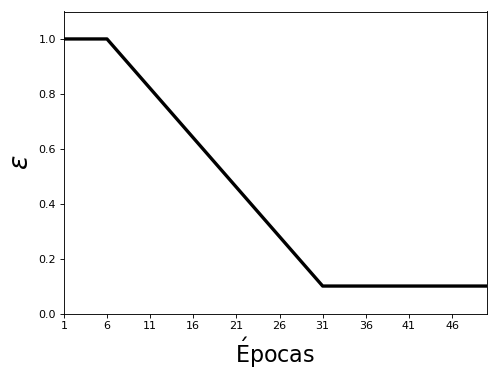
\includegraphics[width=200pt]{epsilon-decay.png}
                    \caption{Fonte:}
                    \label{fig:epsilon-decay}
                \end{figure}
            \end{itemize}
        
        \subsubsection{Índice de Gittins}

\section{Função valor-ação}

    Função valor-ação ótima:

    \begin{equation}
        q_*(a) \ \dot{=} \ \mathbb{E}[R_t \mid A_t = a]
    \end{equation}

    Escolha gulosa:

    \begin{equation}
        A_t \ \dot{=} \ \argmax_a Q_t(a)
    \end{equation}
    
    \begin{center}
    \begin{tikzpicture}[->,>=stealth', auto, node distance=4.0cm, thick]
        \tikzstyle{state}=[fill=none,shape=circle,draw=black,text=black]
        \tikzstyle{action}=[fill=none, draw=none, text=black, shape=circle, inner sep=0,outer sep=0, minimum size=0.0cm]
        \tikzstyle{reward}=[shape=rectangle, text=black, draw=black, fill=white, minimum size=0.5cm, align=center, yshift=0.0cm, anchor=center]
        \tikzstyle{reward-edge}=[text=white, draw=none, fill=none, inner sep=0,outer sep=0, minimum size=0.0cm]
        
        \node[state]  (S1) {$s_1$};
        \node[state]  (S2) [below of=S1, xshift=-3.0cm] {$s_2$};
        \node[state]  (S3) [below of=S1, xshift= 3.0cm] {$s_3$};
        \node[action] (A1) [above of=S2, yshift=-1.5cm] {};
        \node[action] (A2) [below of=S1, yshift=2.5cm]  {};
        
        \draw[bend right=20,-] (S1) to node[above]          {$a_1$} (A1);
        \draw[bend right=30]   (A1) to node[left, pos=0.2]  {$p_1$} (S2);
        \draw[bend left=30]    (A1) to node[right, pos=0.2] {$p_2$} (S2);
        \draw[-]               (S1) to node[pos=0.4]        {$a_2$} (A2);
        \draw[bend left=40]    (A2) to node[left, pos=0.3]  {$p_3$} (S2);
        \draw[bend right=40]   (A2) to node[right, pos=0.3] {$p_4$} (S3);
        \draw[bend left=40]    (S1) to node[above, pos=0.25] {$a_3$} (S3);
        \draw[reward-edge, bend right=30] (A1) to node[reward]           {$r_1$} (S2);
        \draw[reward-edge, bend left=30]  (A1) to node[reward]           {$r_2$} (S2);
        \draw[reward-edge, bend left=40]  (A2) to node[reward]           {$r_3$} (S2);
        \draw[reward-edge, bend right=40] (A2) to node[reward]           {$r_4$} (S3);
        \draw[reward-edge, bend left=40]  (S1) to node[reward, pos=0.65] {$r_5$} (S3);
    \end{tikzpicture}
    \end{center}
    
    \subsection{Definição}
    
    \subsection{Versão incremental}
        
        \begin{equation}
            Q_n \ \dot{=} \ \frac{R_1 + R_2 + \cdots + R_{n-1}}{n - 1}
        \end{equation}
        
        \begin{equation}
        \begin{split}
            Q_{n+1} & \ \dot{=} \ \frac{1}{n} \sum_{i=1}^{n} R_i \\
            & = \ Q_n + \frac{1}{n} \Big[ R_n - Q_n \Big]
        \end{split}
        \end{equation}
        
        Ver no livro a derivação dessa equação (eq. 2.3).
        
        \begin{equation}
            NovaEstimativa \leftarrow AntigaEstimativa + TamanhoPasso \Big[ Objetivo - AntigaEstimativa \Big]
        \end{equation}
        
        \begin{equation}
        \begin{split}
            Q_{n+1} & \ \dot{=} \ Q_n + \alpha \Big[ R_n - Q_n \Big] \\
            & = \ (1 - \alpha)^n Q_1 + \sum_{i=1}^{n} \alpha (1 - \alpha)^{n - i} R_i
        \end{split}
        \end{equation}
        
    \subsection{Escolha dos valores iniciais}
        
        Obs.: citar a diferença entre problemas estacionários e não-estacionários
    
\end{document}
